\documentclass{article}

\usepackage[italian]{babel}

\usepackage{graphicx}
\usepackage{mathtools}
\usepackage{amssymb}
\usepackage{amsthm}
\usepackage{amsmath}
\usepackage{stackengine}
\usepackage{hyperref}
\usepackage{upgreek}
\usepackage{bm}
\usepackage{braket}
\usepackage{cancel}

\newtheorem{axiom}{Assioma}
\newtheorem{defn}{Definizione}
\newtheorem{obs}{Osservazione}
\newtheorem{ex}{Esempio}
\newtheorem{notz}{Notazione}
\newtheorem{corl}{Corollario}
\newtheorem{teo}{Teorema}
\theoremstyle{remark}
\newtheorem{caso}{Caso}

\newcommand{\intR}{\int_{\mathbb{R}}}

\makeindex
\title{\textbf{DISTRIBUZIONI PER ESPERIMENTAZIONI I}}
\author{Manuel Gabriele Moretti}
\date{Settembre 2024}

\begin{document}

\maketitle
\tableofcontents
\newpage

\section{Distribuzione \texorpdfstring{$\chi^2$}{chi-quadro}}
Si definisce la variabile $\chi^2$ come
\begin{equation}
    \chi^2 := \sum_{i=1}^n\chi_i^2,\quad \nu = n.
\end{equation}
Quando $\chi_1,\dots,\chi_n$ sono variabili normali, centrate ed indipendenti, allora la variabile $\chi^2$ risulta essere somma di variabili $\chi^2$. La distribuzione per $\nu = 1$ è
\begin{equation}
    g(\chi^2) = \frac{1}{\sqrt{2\pi}}e^{-\chi^2/2}(\chi^2)^{-1/2} = \frac{1}{2^{1/2}\Gamma(1/2)}e^{-\chi^2/2}(\chi^2)^{(1/2) - 1}.
\end{equation}
In generale, la distribuzione per $\nu = n$ è
\begin{equation}
    g(\chi^2) = \frac{1}{2^{n/2}\Gamma(n/2)}e^{-\chi^2/2}(\chi^2)^{(n/2) - 1}.
\end{equation}
Il valore medio è
\begin{equation}
    \begin{split}
        E[\chi^2]&=\int_0^\infty\chi^2f(\chi^2)d\chi^2 \\
        &=\frac{1}{2^{n/2}\Gamma(n/2)}\int_0^\infty(\chi^2)(\chi^2)^{(n/2) - 1}e^{-\chi^2/2}d\chi^2 \\
        &=\frac{1}{2^{n/2}\Gamma(n/2)}\int_0^\infty(\chi^2)^{n/2}e^{-\chi^2/2}d\chi^2,
    \end{split}
\end{equation}
dove, sostituendo $\chi^2=2t$ e $d\chi^2=2dt$, si ha
\begin{equation}
    \begin{split}
        E[\chi^2] &=\frac{2\cdot2^{n/2}}{2^{n/2}\Gamma(n/2)}\int_0^\infty t^{n/2}e^{-t}dt \\
        &=\frac{2\cdot\cancel{2^{n/2}}}{\cancel{2^{n/2}}\Gamma(n/2)}\Gamma\left(\frac{n}{2}+1\right)\\
        &=\frac{\cancel{2}}{\cancel{\Gamma(n/2)}}\left(\frac{n}{\cancel{2}}\right)\cancel{\Gamma\left(\frac{n}{2}\right)} \\
        &=n.
    \end{split}
\end{equation}
La varianza è
\begin{equation}
    \begin{split}
        E[(\chi^2)^2]&=\int_0^\infty(\chi^2)^2f(\chi^2)d\chi^2 \\
        &=\frac{1}{2^{n/2}\Gamma(n/2)}\int_0^\infty(\chi^2)^2(\chi^2)^{(n/2) - 1}e^{-\chi^2/2}d\chi^2 \\
        &=\frac{1}{2^{n/2}\Gamma(n/2)}\int_0^\infty(\chi^2)^{(n/2)+1}e^{-\chi^2/2}d\chi^2,
    \end{split}
\end{equation}
dove sostituendo $\chi^2=2t$ e $d\chi^2=2dt$, si ha
\begin{equation}
    \begin{split}
        E[(\chi^2)^2] =\frac{2}{2^{n/2}\Gamma(n/2)}\int_0^\infty(2t)^{(n/2)+1}e^{-t}dt &=\frac{2\cdot2^{(n/2)+1}}{2^{n/2}\Gamma(n/2)}\int_0^\infty t^{(n/2)+1}e^{-t}dt\\
        &=\frac{4}{\Gamma(n/2)}\Gamma\left(\frac{n}{2}+2\right) \\
        &=\frac{4}{\Gamma(n/2)}\left(\frac{n}{2}+1\right)\Gamma\left(\frac{n}{2}+1\right) \\
        &=\frac{4}{\cancel{\Gamma(n/2)}}\left(\frac{n}{2}+1\right)\left(\frac{n}{2}\right)\cancel{\Gamma\left(\frac{n}{2}\right)} \\
        &=n^2+2n,
    \end{split}
\end{equation}
da cui si trova
\begin{equation}
    \sigma^2=E[(\chi^2)^2]-(E[\chi^2])^2=n^2+2n-n^2=2n.
\end{equation}
La moda è data da 
\begin{equation}
    \frac{df(\chi^2)}{d\chi^2}=\frac{1}{\cancel{2^{n/2}\Gamma\left(n/2\right)}}\left[\left(\frac{n}{2}-1\right)(\chi^2)^{(n/2) - 2}\cancel{e^{-\chi^2/2}}-\frac{1}{2}(\chi^2)^{(n/2) - 1}\cancel{e^{-\chi^2/2}}\right]=0,
\end{equation}
da cui si trova che la moda si ha per 
\begin{equation}
        \left(\frac{n}{2}-1\right)\frac{\cancel{(\chi^2)^{(n/2) - 1}}}{\chi^2}=\frac{1}{2}\cancel{(\chi^2)^{(n/2) - 1}} \quad \Longrightarrow \quad \chi^2=n-2.
\end{equation}

\section{Distribuzione \texorpdfstring{$W$}{W}}
Si definisce la variabile $W$ come
\begin{equation}
    W := \frac{\sum\nolimits_i\chi^2}{n} \equiv \tilde{\chi}^2.
\end{equation}
Per cui la distribuzione è
\begin{equation}
    g(W)dW = f(\chi^2)d\chi^2,
\end{equation}
da cui, sostituendo $\chi^2=nW$ e $d\chi^2=ndW$, si ha
\begin{equation}
    \begin{split}
        g(W)\cancel{dW}&=\frac{1}{2^{n/2}\Gamma(n/2)}(nW)^{(n/2) - 1}e^{-nW/2}n\cancel{dW}\\
        &=\frac{\left(n/2\right)^{n/2}}{\Gamma(n/2)}W^{(n/2) - 1}e^{-nW/2}.
    \end{split}
\end{equation}
Il valore atteso è
\begin{equation}
    E[W]=E\left[\frac{\chi^2}{n}\right]=\frac{1}{n}E[\chi^2]=\frac{n}{n}=1.
\end{equation}
La varianza è data da
\begin{equation}
    \sigma^2=E[W^2]-(E[W])^2=E[W^2]-1.
\end{equation}
Calcolando
\begin{equation}
    E[W^2]=E\left[\left(\frac{\chi^2}{n}\right)^2\right]=\frac{1}{n^2}E[(\chi^2)^2]=\frac{1}{n^2}(n^2+2n)=1+\frac{2}{n},
\end{equation}
si trova
\begin{equation}
    \sigma^2=1+\frac{2}{n}-1=\frac{2}{n}.
\end{equation}

\section{Distribuzione \texorpdfstring{$r$}{r}}
Si definisce la variabile $r$ come
\begin{equation}
    r = \sqrt{W} = \sqrt{\tilde{\chi}^2}.
\end{equation}
Se $\chi^2 = nr$, allora $d\chi^2 = 2nr\,dr$ e
\begin{equation}
    \begin{split}
        g(r)\,\cancel{dr} &= f(\chi^2)\,d\chi^2 \\
        &= \frac{1}{2^{n/2}\Gamma(n/2)}(nr^2)^{(n/2) - 1}e^{-nr^2/2}2nr\,dr \\
        &= \frac{2n}{2^{n/2}\Gamma(n/2)}n^{(n/2) - 1}r(r^2)^{(n/2) - 1}e^{-nr^2/2}\,dr \\
        &= \frac{2n}{2^{n/2}\Gamma(n/2)}n^{n/2}\frac{\cancel{r}r^n}{r^{\cancel{2}}}e^{-nr^2/2}\,dr \\
        &= \frac{2(n/2)^{n/2}}{\Gamma(n/2)}r^{n - 1}e^{-nr^2/2}\,\cancel{dr}.
    \end{split}
\end{equation}
Il valore atteso è dato da
\begin{equation}
    E[r] = \int_0^\infty rg(r)\,dr = \frac{2(n/2)^{n/2}}{\Gamma(n/2)}\int_0^\infty r^ne^{-nr^2/2}\,dr.
\end{equation}
Sostituendo $nr^2/2 = t$ e $dr = dt/\sqrt{2nt}$, si ha
\begin{equation}
    \begin{split}
        E[r] &= \frac{2(n/2)^{n/2}}{\Gamma(n/2)}\int_0^\infty \bigg(\sqrt{\frac{2t}{n}}\bigg)^{n}e^{-t}\frac{1} {\sqrt{2nt}}\,dt \\
        &= \frac{2\cancel{(n/2)^{n/2}}}{\Gamma(n/2)}\cancel{\bigg(\sqrt{\frac{2}{n}}\bigg)^{n}}\frac{1}{\sqrt{2n}}\int_0^\infty t^{(n - 1)/2}e^{-t}\,dt \\
        &= \frac{2}{\Gamma(n/2)}\frac{1}{\sqrt{2n}}\Gamma\bigg(\frac{n - 1}{2} + 1\bigg) \\
        &= \frac{2}{\Gamma(n/2)}\frac{1}{\sqrt{2n}}\Gamma\bigg(\frac{n + 1}{2}\bigg).
    \end{split}
\end{equation}
La varianza è data da
\begin{equation}
    E[r^2] = \int_0^\infty r^2g(r)\,dr = \frac{2(n/2)^{n/2}}{\Gamma(n/2)}\int_0^\infty r^{n + 1}e^{-nr^2/2}\,dr.
\end{equation}
Sostituendo $nr^2/2 = t$ e $dr = dt/\sqrt{2nt}$, si ha
\begin{equation}
    \begin{split}
        E[r^2] &= \int_0^\infty r^2g(r)\,dr \\
        &= \frac{2(n/2)^{n/2}}{\Gamma(n/2)}\int_0^\infty \bigg(\sqrt{\frac{2t}{n}}\bigg)^{n + 1}e^{-t}\frac{1}{\sqrt{2nt}}\,dr \\
        &= \frac{2(n/2)^{n/2}}{\Gamma(n/2)}\bigg(\sqrt{\frac{2}{n}}\bigg)^{n + 1}\frac{1}{\sqrt{2n}}\int_0^\infty t^{n/2}e^{-t}\,dr \\
        &= \frac{2(\cancel{(n/2)^{n/2}}}{\cancel{\Gamma(n/2)}}\cancel{\bigg(\sqrt{\frac{2}{n}}\bigg)^{n}}\bigg(\sqrt{\frac{2}{n}}\bigg)^n\frac{1}{\sqrt{2n}}\frac{n}{2}\cancel{\Gamma\bigg(\frac{n}{2}\bigg)} \\
        &= 1
    \end{split}
\end{equation}
da cui si trova che la varianza è
\begin{equation}
    Var[r] = 1 - \bigg[\frac{2}{\Gamma(n/2)\sqrt{2n}}\Gamma\bigg(\frac{n + 1}{2}\bigg)\bigg]^2.
\end{equation}

\section{Distribuzione \texorpdfstring{$t$}{t} di Student}
Si fissa $r$ con $z = rt$, da cui $dz = r\,dt$ e quindi
\begin{equation}
    \bigg|\frac{dz}{dt}\bigg| = r.
\end{equation}
Si determina la funzione di densità di probabilità condizionata come
\begin{equation}
    \phi(t|r) = r f(rt) = \frac{1}{\sqrt{2\pi}}e^{-(rt)^2/2}r,\quad t \in (-\infty,\infty).
\end{equation}
Si determina la funzione di densità di probabilità congiunta come
\begin{equation}
    \begin{split}
        d(r,t) = \phi(t|r)g(r) &= \frac{1}{\sqrt{2\pi}}e^{-(rt)^2/2}r\bigg[\bigg(\frac{n}{2}\bigg)^{n/2}\frac{2r^{n - 1}}{\Gamma(n/2)}e^{-nr^2/2}\bigg] \\
        &= \frac{2(n/2)^{n/2}}{\sqrt{2\pi}\Gamma(n/2)}r^ne^{-(n + t^2)r^2/2} \\
        &= C(n)r^ne^{-nr^2(1 + t^2/n)/2},
    \end{split}
\end{equation}
con $r \in [0,\infty)$. Si integra su $r$ per definire
\begin{equation}
    h(t) = \int_0^\infty C(n)r^n e^{-n(1 + t^2/n)r^2/2}\,dr.
\end{equation}
Poi, tramite il cambio di variabili $u = r\sqrt{(t^ 2 + n)/2}$ che restituisce 
\begin{equation}
    r = \frac{u\sqrt{2}}{\sqrt{t^2 + n}},\quad dr = \sqrt{\frac{u}{n + t^2}}\,du,
\end{equation}
si ha
\begin{equation}
    \begin{split}
        h(t) &= \int_0^\infty C(n)\bigg(u\sqrt{\frac{2}{t^2 + n}}\bigg)^ne^{-u^2}\sqrt{\frac{2}{t^2 + n}}\,du \\
        &= C(n)\bigg(\sqrt{\frac{2}{t^2 + n}}\bigg)^n\int_0^\infty u^ne^{-u^2}\,du,
    \end{split}
\end{equation}
da cui, sostituendo $q = u^2$ e $du = dq/(2\sqrt{q})$, si ottiene
\begin{equation}
    \begin{split}
        h(t) &= C'(n)\int_0^\infty q^{(n - 1)/2}e^{-q}\,dq \\
        &= C'(n)\Gamma\bigg(\frac{n + 1}{2}\bigg) \\ 
        &= \frac{1}{\Gamma(n/2)\sqrt{n\pi}(1 + t^2/n)^{(n + 1)/2}}\Gamma\bigg(\dfrac{n + 1}{2}\bigg).
    \end{split}
\end{equation}
Dunque, $h(t)$ dipende da $n$ gradi di libertà ed è simmetrica, ossia $E[t] = 0$. Ha varianza $n/(n - 2)$, per cui se $n \to \infty$ la varianza tende ad 1 come per la normale standardizzata. Il valore atteso è 
\begin{equation}
    E[t] = E\bigg[\frac{z}{r}\bigg] = E[z]E\bigg[\frac{1}{r}\bigg] = 0.
\end{equation}
La varianza è data da
\begin{equation}
    Var[t] = E[t^2] - (E[t])^2 = E\bigg[\frac{z^2}{r^2}\bigg] = E[z^2]E\bigg[\frac{1}{r^2}\bigg] = E\bigg[\frac{n}{\chi^2}\bigg] =nE\bigg[\frac{1}{\chi^2}\bigg].
\end{equation}
Calcolando
\begin{equation}
    \begin{split}
        E\bigg[\frac{1}{\chi^2}\bigg] &= \frac{1}{2^{n/2}\Gamma(n/2)}\int_0^\infty(\chi^2)^{-1}(\chi^2)^{(n/2) - 1}e^{-\chi^2/2}\,d\chi^2 \\
        &= \frac{1}{2^{n/2}\Gamma(n/2)}\int_0^\infty(\chi^2)^{(n/2) - 2}e^{-\chi^2/2}\,d\chi^2,
    \end{split}
\end{equation}
da cui, sostituendo $\chi^2/2 = y^2$, $d\chi^2 = 2dy$, si ha
\begin{equation}
    \begin{split}
        E\bigg[\frac{1}{\chi^2}\bigg] = \frac{2^{(n/2) - 2}}{2^{n/2}\Gamma(n/2)}2\int_0^\infty y^{(n/2) - 2}e^{-y} &= \frac{1}{2\Gamma(n/2)}\Gamma\bigg(\frac{n}{2} - 1\bigg) \\
        &= \frac{1}{2((n/2) - 1)\cancel{\Gamma((n/2)- 1)}}\cancel{\Gamma\bigg(\frac{n}{2} - 1\bigg)} \\
        &= \frac{1}{n - 2}.
    \end{split}
\end{equation}
Dunque, la varianza è
\begin{equation}
    Var[t] = \frac{n}{n - 2}.
\end{equation}

\section{Distribuzione \texorpdfstring{$F$}{F} di Fisher}
La variabile $F$ è definita come rapporto tra due variabili $W$, ossia 
\begin{equation}
    F := \frac{\chi_1^2/\nu_1}{\chi_2^2/\nu_2}\frac{\nu_2\chi_1^2}{\nu_1\chi_2^2} \equiv \frac{b}{a}\frac{r}{s}.
\end{equation}
Quindi è possibile confrontare due relazioni funzionali diverse associate agli stessi dati e scegliere tra due fit diversi dai i valori di $\chi^2$. Si fissi $s$ con $r = asF/b$, da cui
\begin{equation}
    dr = \frac{as}{b}\,dF.
\end{equation}
Si determina la funzione di probabilità condizionata come
\begin{equation}
    \phi(F|s) = \frac{1}{2^{a/2}\Gamma(a/2)}\bigg(\frac{a}{b}sF\bigg)^{(a/2) - 1}\frac{as}{b}.
\end{equation}
Si determina la funzione di probabilità congiunta come
\begin{equation}
    g(F,s) = \phi(F|s)g(s).
\end{equation}
Si integra su $s$ per definire
\begin{equation}
    h(F) = \int_0^\infty g(F,s)\,ds = \frac{\Gamma\bigg(\dfrac{\nu_1}{2} + \dfrac{\nu_2}{2}\bigg)}{\Gamma\bigg(\dfrac{\nu_1}{2}\bigg) + \Gamma\bigg(\dfrac{\nu_2}{2}\bigg)}\bigg[\frac{(\nu_1F)^{\nu_1}\nu_2^{1/2}}{(\nu_1F + \nu_2)^{\nu_1 + \nu_2}}\bigg]\frac{1}{F}.
\end{equation}
Il valore atteso è
\begin{equation}
    E[F] = E\bigg[\frac{b}{a}\frac{\chi_1^2}{\chi_2^2}\bigg] = \frac{b}{a}E\bigg[\frac{\chi_1^2}{\chi_2^2}\bigg] = \frac{ba}{a(b - 2)} = \frac{b}{b - 2},
\end{equation}
il quale esiste se e solo se $\nu_b = 2$. La varianza è data da
\begin{equation}
    \sigma_F^2 = E[F^2] - (E[F])^2 = E[F^2] - \bigg(\frac{b}{b - 2}\bigg)^2.
\end{equation}
Calcolando
\begin{equation}
    E[F^2] = E\bigg[\bigg(\frac{b}{a}\frac{\chi_1^2}{\chi_2^2}\bigg)^2\bigg] = \frac{b^2}{a^2}E[(\chi_1^2)^2]E\bigg[\bigg(\frac{1}{\chi_2^2}\bigg)^2\bigg],
\end{equation}
dove 
\begin{equation}
    E[(\chi_1^2)^2] = \sigma_{\chi^2}^2 + (E[\chi^2])^2 = 2a + a^2 = a(a + 2),
\end{equation}
\begin{equation}
    E\bigg[\bigg(\frac{1}{\chi_2^2}\bigg)^2\bigg] = \int_0^\infty(\chi_2^2)^{-2}f(\chi^2)\,d\chi^2 = \frac{1}{(b - 2)(b - 4)},
\end{equation}
si ottiene che la varianza è
\begin{equation}
    \sigma_F^2 = \frac{b^2}{a^{\cancel{2}}}a(a + 2)\frac{1}{(b - 2)(b - 4)} - \bigg(\frac{b}{b - 2}\bigg)^2,
\end{equation}
la quale esiste se e solo se $\nu_b > 4$.

\section{Distribuzione gaussiana}
La densità di probabilità è
\begin{equation}
    f(x) = \frac{1}{\sqrt{2\pi}\sigma}\exp{\bigg[\frac{(x - \mu)^2}{2\sigma^2}\bigg]}.
\end{equation}
Ponendo $z = (x - \mu)/\sigma$ si ha $dz = dx/\sigma$, per cui
\begin{equation}
    f(x)\,dx = \frac{1}{\sqrt{2\pi}\sigma}e^{-z^2/2}\sigma dz = g(x)\,dz,\quad g(z) \equiv \frac{1}{\sqrt{2\pi}\sigma}e^{-z^2/2}.
\end{equation}
Si definisce la funzione di ripartizione della distribuzione normale (o gaussiana) ridotta come
\begin{equation}
    F(z) := \int_{-\infty}^0 g(z)\,dz,
\end{equation}
dove la funzione $g(z)$ ha le seguenti proprietà:
\begin{enumerate}
    \item è continua su $(-\infty,\infty)$;
    \item è pari, ossia vale che $g(z) = g(-z)$;
    \item il massimo si ha per $g(0) = 1/\sqrt{2\pi} \equiv g_{max}$;
    \item $g(z) \to 0$ per $x \to \pm\infty$.
\end{enumerate}
La derivata di $g(z)$ è
\begin{equation}
    g'(z) = -\frac{z}{\sqrt{2\pi}}e^{-z^2/2},
\end{equation}
dove se:
\begin{enumerate}
    \item $z < 0$, allora $g'(z) > 0$, ossia $g(z)$ è crescente su $[-\infty,0]$;
    \item $z > 0$, allora $g'(z) < 0$, ossia $g(z)$ decrescente su $[0,\infty]$.
\end{enumerate}
La derivata seconda di $g(z)$ è
\begin{equation}
    g''(z) = \frac{dg'}{dz} = -\frac{1}{\sqrt{2\pi}}\bigg[e^{-z^2/2} + z\bigg(-\frac{1}{2}2ze^{-z^2/2}\bigg)\bigg] = -\frac{e^{-z^2/2}}{\sqrt{2\pi}}(1 - z^2),
\end{equation}
dove i punti di flesso sono dati da 
\begin{equation}
    g''(z) = 0 \quad \Longrightarrow \quad 1 - z^2 = 0 \quad \Longrightarrow \quad z_{F} = \pm 1.
\end{equation}
Inoltre, valutando $g(z)$ nei punti di flesso si ha
\begin{equation}
    g(z_{F}) = g(\pm 1) = \frac{1}{\sqrt{2\pi}}e^{-1/2} = \frac{1}{\sqrt{2\pi e}} = \frac{1}{\sqrt{e}}g_{max}.
\end{equation}
Se $x = \mu + z\sigma$, allora per $z = 0$ si ha $x = \mu$ e per $z = \pm 1$ si ha $x = \mu \pm \sigma$. 

Si può dimostrare che se $g(z) = C e^{-z^2/2}$, allora $C = 1/\sqrt{2\pi}$. Per farlo, si parte dal fatto che 
\begin{equation}
    I_G = \intR e^{y^2}\,dy = \sqrt{\pi}.
\end{equation}
Usando il cambio di variabili $z = \sqrt{2}y$ con $dy = dz/\sqrt{2}$, si ha che 
\begin{equation}
    \sqrt{2}I_G \equiv I_G' = \intR e^{-z^2/2}\,dz = \sqrt{2\pi}.
\end{equation}
Imponendo la condizione di normalizzazione su $g(z)$,
\begin{equation}
    \intR g(z)\,dz = 1,
\end{equation}
si ha
\begin{equation}
    \intR Ce^{-z^2/2}\,dz = C\sqrt{2\pi} = 1 \Longrightarrow C = \frac{1}{\sqrt{2\pi}},
\end{equation}
come volevasi dimostrare. Il valore atteso è dato da
\begin{equation}
    E[x] = \intR xf(x)\,dx = \frac{1}{\sqrt{2\pi}\sigma}\intR x\exp{\bigg[-\frac{(x - \mu)^2}{2\sigma^2}\bigg]}\,dx.
\end{equation}
Usando $z = (x - \mu)/\sigma$, si ha
\begin{equation}
    \begin{split}
        E[x] &= \frac{1}{\sqrt{2\pi}\cancel{\sigma}}\intR\cancel{\sigma}(\mu + \sigma z)e^{-z^2/2}\,dz \\
        &= \frac{1}{\sqrt{2\pi}}\bigg[\mu\underbrace{\intR e^{-z^2/2}\,dz}_{I_G = \sqrt{2\pi}} + \sigma\bigg(\underbrace{\intR ze^{-z^2/2}\,dz}_{=\,0,\,h(z)\,\mathrm{dispari}}\bigg)\bigg] \\
        &= \mu.
    \end{split}
\end{equation}
Tramite l'integrale 
\begin{equation}
    I_u = \intR u^2e^{-u^2}\,du = -\frac{1}{2}\intR ud(e^{-u^2}) = -\frac{1}{2}\bigg([ue^{-u^2}]_{\mathbb{R}} - \intR e^{-u^2}\,du\bigg) = \frac{\sqrt{\pi}}{2},
\end{equation}
dove si è usato che $d(e^{-u^2}) = 2ue^{-u^2}\,du$, si trova che la varianza è data da
\begin{equation}
    \begin{split}
        Var[x] = E[(x - \mu)^2] &= \intR (x - \mu)^2f(x)\,dx \\
        &= \frac{1}{\sqrt{2\pi}\sigma}\intR(x - \mu)^2\exp{\bigg[-\frac{(x - \mu)^2}{2\sigma^2}\bigg]}\,dx,
    \end{split}
\end{equation}
da cui, sostituendo prima $z = (x - \mu)/\sigma$, si ha
\begin{equation}
    \begin{split}
        Var[x] &= \frac{1}{\sqrt{2\pi}\cancel{\sigma}}\intR\cancel{\sigma}(\sigma z)^2e^{-z^2/2}\,dz \\
        &= \frac{\sigma^2}{\sqrt{2\pi}}\intR z^2e^{-z^2/2}\,dz,
    \end{split}
\end{equation}
mentre, sostituendo $u = z/\sqrt{2}$, si ha
\begin{equation}
    \begin{split}
        Var[x] = \frac{\sigma^2}{\sqrt{\cancel{2}\pi}}\intR 2u^2e^{-u^2}\cancel{\sqrt{2}}\,du &= \frac{2\sigma^2}{\sqrt{\pi}}\intR u^2e^{-u^2/2}\,du \\
        &= \frac{2\sigma^2}{\sqrt{\pi}}\frac{\sqrt{\pi}}{2} \\
        &= \sigma,
    \end{split}
\end{equation}
Si definisce la ``Full Width at Half Maximum'' (FWHM) come
\begin{equation}
    \mathrm{FWHM} := x_2 - x_1,\quad f(x_1) = f(x_2) = \frac{1}{2}f_{max},
\end{equation}
come si vede in figura \ref{fig: FWHM}. Per determinarne il valore, si parte da
\begin{equation}
    \begin{split}
        f(x) = \cancel{f_{max}}\exp{\bigg[-\frac{(x - \mu)^2}{2\sigma^2}\bigg]} &= \frac{1}{2}\cancel{f_{max}} \\
        -\frac{(x - \mu)^2}{2\sigma^2} &= -\ln{2} \\
        (x - \mu)^2 &= 2\ln{(2)}\sigma^2,
    \end{split}
\end{equation}
da cui si definisce la ``Half Width at Half Maximum'' (HWHM) come
\begin{equation}
    \mathrm{HWHM} := |x  - \mu| = \sqrt{2\ln{2}}\sigma,
\end{equation}
con la quale si trova che 
\begin{equation}
    \mathrm{FWHM} = 2\sqrt{2\ln{2}}\sigma.
\end{equation}
\begin{figure}[h]
    \centering
    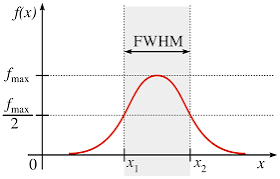
\includegraphics[width=0.4\linewidth]{Immagini/FWHM.png}
    \caption{la definizione della FWHM.}
    \label{fig: FWHM}
\end{figure}

\end{document}
